%\VignetteIndexEntry{MeSH.db}
\documentclass[11pt]{article}
\usepackage{Sweave}
\usepackage{amsmath}
\usepackage{hyperref}
\usepackage{cite}
\usepackage{Sweave}

\usepackage[numbers]{natbib}
\usepackage{amsmath}
\usepackage{amssymb}
\input{MeSH-concordance}
\usepackage{hyperref,url}
\usepackage[utf8]{inputenc}
\usepackage{comment}

\setlength{\textheight}{8.5in}
\setlength{\textwidth}{6in}
\setlength{\topmargin}{-0.25in}
\setlength{\oddsidemargin}{0.25in}
\setlength{\evensidemargin}{0.25in}
\newcommand{\Rpackage}[1]{{\textit{#1}}}

\usepackage{Sweave}
\begin{document}


\title{\bf How to use MeSH-related Packages}
\author{Koki Tsuyuzaki$^{1,4}$, Gota Morota$^2$, Takeru Nakazato$^3$ and Itoshi Nikaido$^4$.}
\maketitle
\begin{center}
\noindent
$^1$Department of Medical and Life Science, Tokyo University of Science.\\
\noindent
$^2$Department of Animal Science, University of Nebraska-Lincoln\\
\noindent
$^3$Database Center for Life Science, Research Organization of Information and Systems.\\
\noindent
$^4$Bioinformatics Research Unit, RIKEN Advanced Center for Computing and Communication.\\
\end{center}

\begin{center}
{\tt k.t.the-answer@hotmail.co.jp, dritoshi@gmail.com}
\end{center}
\tableofcontents

%%%%%%%%%%%%%%%%%%%%%%%%%%%%%%%%%%%%%%%%%%%%%%%%%%%%%%%%%%%%%%%%%%
%\clearpage
\newpage
\section{Introduction}
This document provides the way to use MeSH-related packages; \Rpackage{MeSH.db}, \Rpackage{MeSH.AOR.db}, \Rpackage{MeSH.PCR.db}, $org.MeSH.XXX.db$-type packages, \Rpackage{MeSHDbi}, and \Rpackage{meshr} packages. MeSH (Medical Subject Headings) is the NLM (U. S. National Library of Medicine) controlled vocabulary used to manually index articles for MEDLINE/PubMed \cite{Nelson2004} and is a collection of a comprehensive life science vocabulary.
%%%%%%%%%%%%%%%%%%%%%%%%%%%%%%%%%%%%%%%%%%%%%%%%%%%%%%%%%%%%%%%%%%
\begin{figure}[ht]
\centering
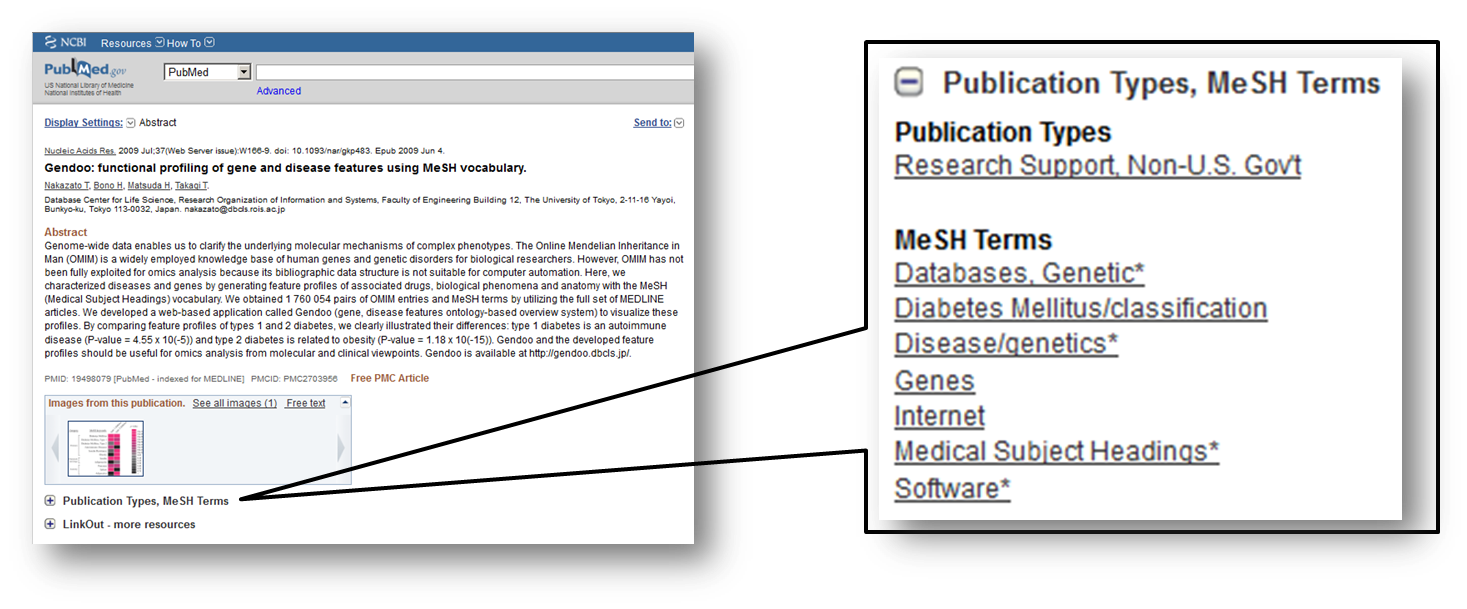
\includegraphics[width=\linewidth]{fig1.png}
\caption{MeSH Term}
\label{fig1}
\end{figure}
%%%%%%%%%%%%%%%%%%%%%%%%%%%%%%%%%%%%%%%%%%%%%%%%%%%%%%%%%%%%%%%%%%
MeSH contains more than 25,000 clinical and biological terms. The amount of MeSH term is about twice as large as that of GO (Gene Ontology)\cite{Ashburner2000} and its categories are also wider. MeSH in 2014 proposed its 19 categories and \Rpackage{MeSH.db} provides 16 of them, which are actually assigned to some MeSH terms. Each category is expressed as single capital alphabet as abbreviation defined by NLM. Therefore MeSH is an expected to be much detailed and exhaustive gene annotation tool. Some software or databases using MeSH are now proposed \cite{Nakazato2007, Nakazato2009, Saurin2010, Sartor2012}.
%%%%%%%%%%%%%%%%%%%%%%%%%%%%%%%%%%%%%%%%%%%%%%%%%%%%%%%%%%%%%%%%%%
\begin{center}
  \begin{table}[htbp]
    \begin{tabular}{|c|l|}\hline
      Abbreviation & Category \\ \hline \hline
      A & Anatomy \\ \hline
      B & Organisms \\ \hline
      C & Diseases \\ \hline
      D & Chemicals and Drugs \\ \hline
      E & Analytical, Diagnostic and Therapeutic Techniques and Equipment \\ \hline
      F & Psychiatry and Psychology \\ \hline
      G & Phenomena and Processes \\ \hline
      H & Disciplines and Occupations \\ \hline
      I & Anthropology, Education, Sociology and Social Phenomena \\ \hline
      J & Technology and Food and Beverages \\ \hline
      K & Humanities \\ \hline
      L & Information Science \\ \hline
      M & Persons \\ \hline
      N & Health Care \\ \hline
      V & Publication Type \\ \hline
      Z & Geographical Locations \\ \hline
\end{tabular}
  \end{table}
\end{center}
%%%%%%%%%%%%%%%%%%%%%%%%%%%%%%%%%%%%%%%%%%%%%%%%%%%%%%%%%%%%%%%%%%
This vignette introduces R/Bioconductor packages for handling MeSH in R. Original MeSH data is accessible by NLM FTP site (\url{http://www.nlm.nih.gov/mesh/filelist.html}). The data are downloadable as plain-text format (ASCII MeSH; d2014.bin / q2014.bin). These files were pre-processed by our data-processing pipeline (figure 2) and corresponding information is summarized as a table in SQLite3 file and packed into \Rpackage{MeSH.db}, \Rpackage{MeSH.AOR.db}, and \Rpackage{MeSH.PCR.db}.

\clearpage
\subsection{About MeSH}
\Rpackage{MeSH.db} provides the corresponding table which contains MeSH ID, MeSH term, MeSH category, synonym, qualifier ID, and qualifier term. Qualifier term means more rough annotation (subheadings) than MeSH. MeSH has hierarchical structure like GO. Such structure is provided as \Rpackage{MeSH.AOR.db} (AOR: ancestor-offspring Relationships) and \Rpackage{MeSH.PCR.db} (PCR: parent-child Relationships as corresponding table.
%%%%%%%%%%%%%%%%%%%%%%%%%%%%%%%%%%%%%%%%%%%%%%%%%%%%%%%%%%%%%%%%%%
\begin{figure}[ht]
\centering
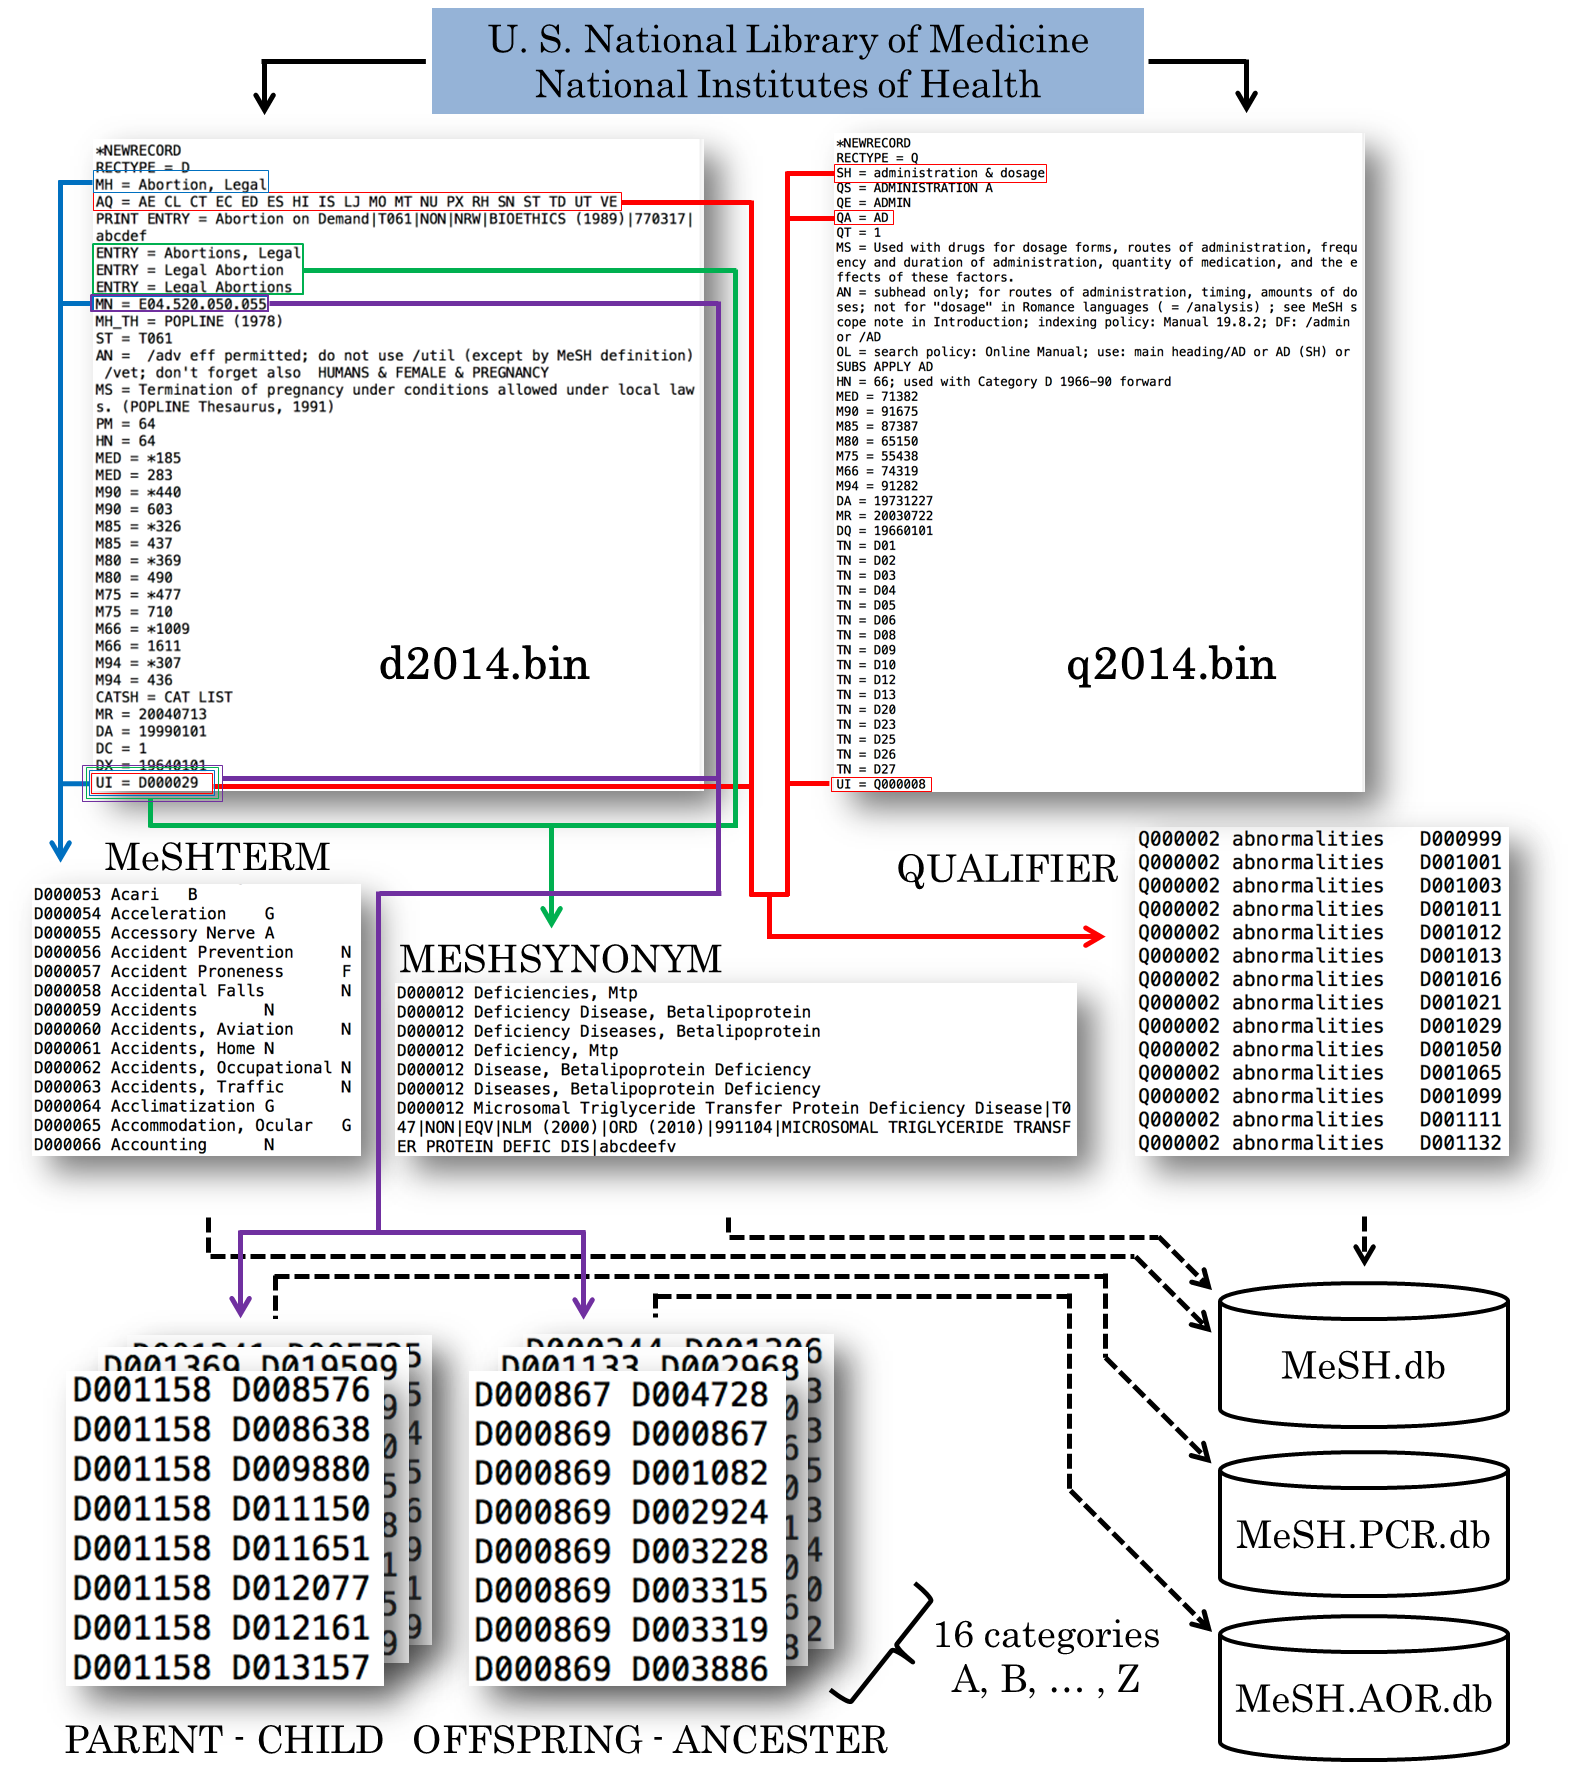
\includegraphics[width=14.0cm]{fig2.png}
\caption{Data pre-process for MeSH.db}
\label{fig2}
\end{figure}
%%%%%%%%%%%%%%%%%%%%%%%%%%%%%%%%%%%%%%%%%%%%%%%%%%%%%%%%%%%%%%%%%%
\clearpage
\subsection{The correspondence between MeSH ID and NCBI Entrez Gene ID}
org.MeSH.XXX.db (XXX is an abbreviation of species name such as Hsa: Homo sapiens) packages provide the correspondence between Entrez Gene IDs and NLM MeSH IDs. Such correspondence in wide variety of organisms are summarized as each org.MeSH.XXX.db by three way of methods, Gendoo\cite{Nakazato2009}, gene2pubmed, and RBBH (reciprocal BLAST best Hit).

Gendoo is the web-application based on text-mining of PubMed. Co-occurrence relations in PubMed document are exhaustively retrieved and much relevant correspondence are filtered by some information science techniques.

gene2pubmed is the correspondence between Entrez Gene IDs and NLM PubMed IDs. These relationship is manually assigned by NCBI curator teams. We also summarized the relationship between MeSH Terms and PubMed IDs from licensed-PubMed, then merged as Gene IDs - MeSH IDs correspondence.

For some minor species including non-model organisms, which have no sufficient databases for annotation, we defined 15 well-annotated organisms and 100 minor-organisms, then conducted RBBH between all possible combinations using BLASTP search.
%%%%%%%%%%%%%%%%%%%%%%%%%%%%%%%%%%%%%%%%%%%%%%%%%%%%%%%%%%%%%%%%%%
\begin{center}
  \begin{table}[htbp]
    \begin{tabular}{|c|l|}\hline
      Method & Way of corresponding Entrez Gene IDs and MeSH IDs \\ \hline \hline
      Gendoo & Text-mining \\ \hline
      gene2pubmed & Manual curation by NCBI teams \\ \hline
      RBBH & sequence homology with BLASTP search (E-value < $10^{-50}$) \\ \hline
\end{tabular}
  \end{table}
\end{center}
%%%%%%%%%%%%%%%%%%%%%%%%%%%%%%%%%%%%%%%%%%%%%%%%%%%%%%%%%%%%%%%%%%

%%%%%%%%%%%%%%%%%%%%%%%%%%%%%%%%%%%%%%%%%%%%%%%%%%%%%%%%%%%%%%%%%%
\begin{figure}[ht]
\centering
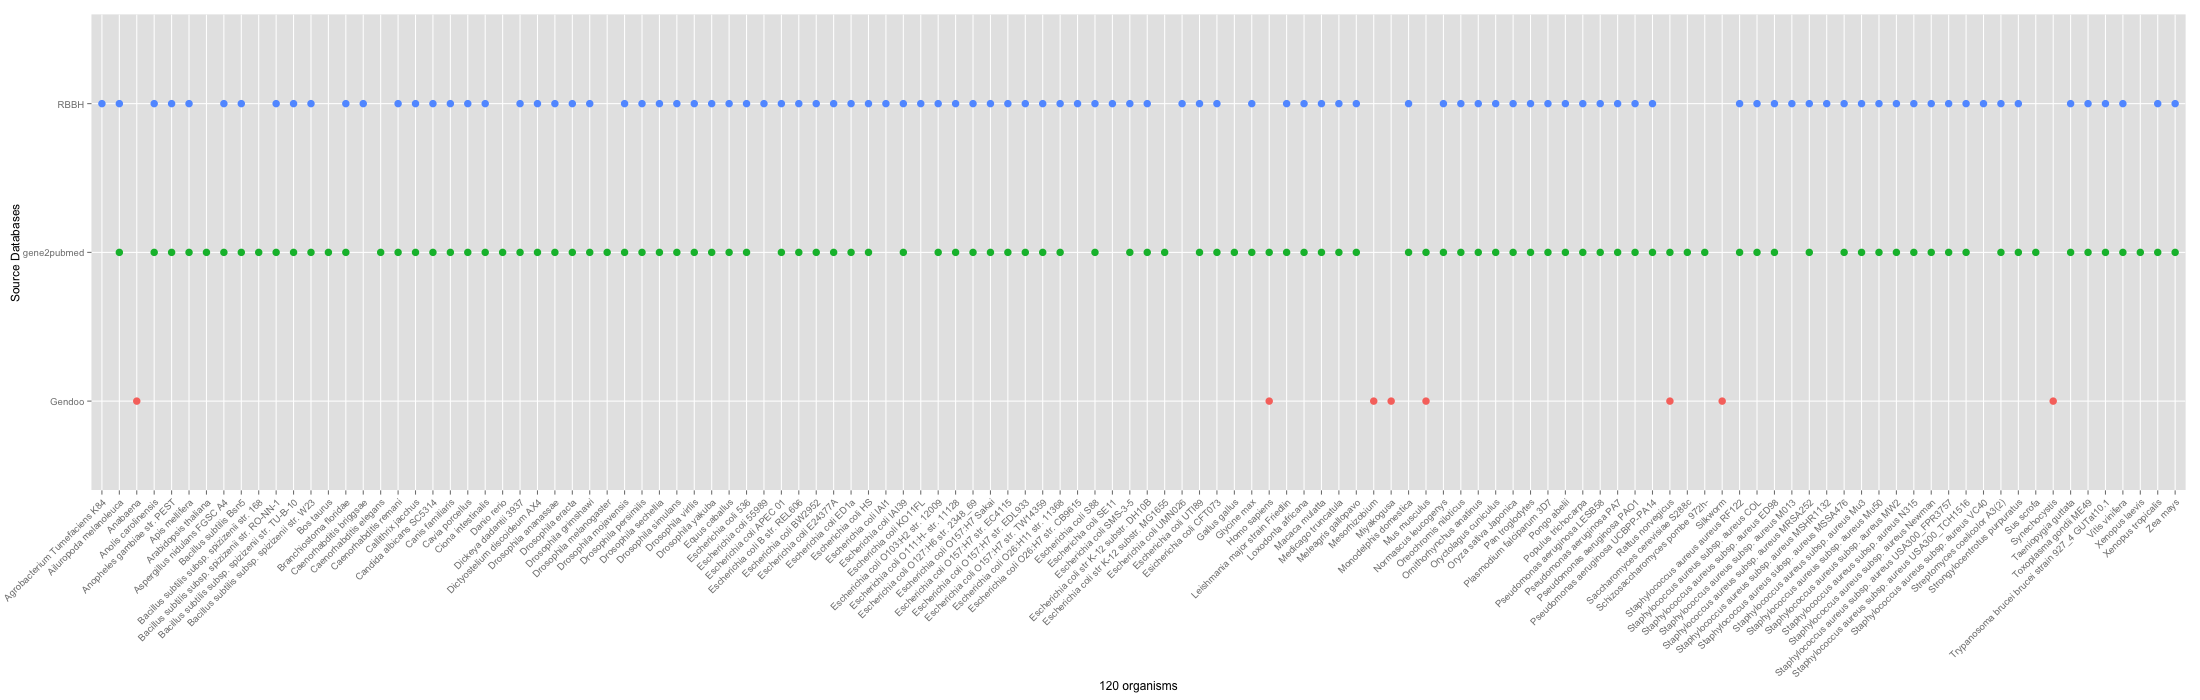
\includegraphics[width=\linewidth,angle=270]{fig3.png}
\caption{120 organisms for org.MeSH.XXX.db and those source databases}
\label{fig3}
\end{figure}
%%%%%%%%%%%%%%%%%%%%%%%%%%%%%%%%%%%%%%%%%%%%%%%%%%%%%%%%%%%%%%%%%%
\clearpage
\subsection{Database interface package for MeSH-related packages}
We also implemented a database interface (DBI) package named \Rpackage{MeSHDbi}. This package is important because of two reasons. First reason is a unification of DBI functions for MeSH-related packages. \Rpackage{MeSH.db}, \Rpackage{MeSH.AOR.db}, \Rpackage{MeSH.PCR.db}, and $org.MeSH.XXX.db$ packages inherit the MeSHDb-class defined by \Rpackage{MeSHDbi} and behavior of these packages is uniformly designed. Second reason is supporting construction of user's original org.MeSH.XXX.db package. Due to the rapid development of DNA sequence technology, wide variety of genome sequences are more and more determined and the correspondence of Gene IDs and MeSH IDs may be designed by many databases \cite{Nakazato2007, Nakazato2009, Saurin2010, Sartor2012}. Therefore, we prepared the function to create org.MeSH.XXX.db package for a situation in which users can retrieved the relationship between Gene IDs and MeSH IDs by some means.

\subsection{MeSH term enrichment analysis}
To analyze MeSH-related packages with omics data, we implement \Rpackage{meshr} package, which is for conducting enrichment analysis using MeSH data. This package internally imports \Rpackage{MeSH.db}, \Rpackage{MeSH.AOR.db}, \Rpackage{MeSH.PCR.db} and $org.MeSH.XXX.db$, then conducts enrichment analysis to detect highlly enriched MeSH terms in gene sets of interesting species.
%%%%%%%%%%%%%%%%%%%%%%%%%%%%%%%%%%%%%%%%%%%%%%%%%%%%%%%%%%%%%%%%%%
\begin{figure}[ht]
\centering
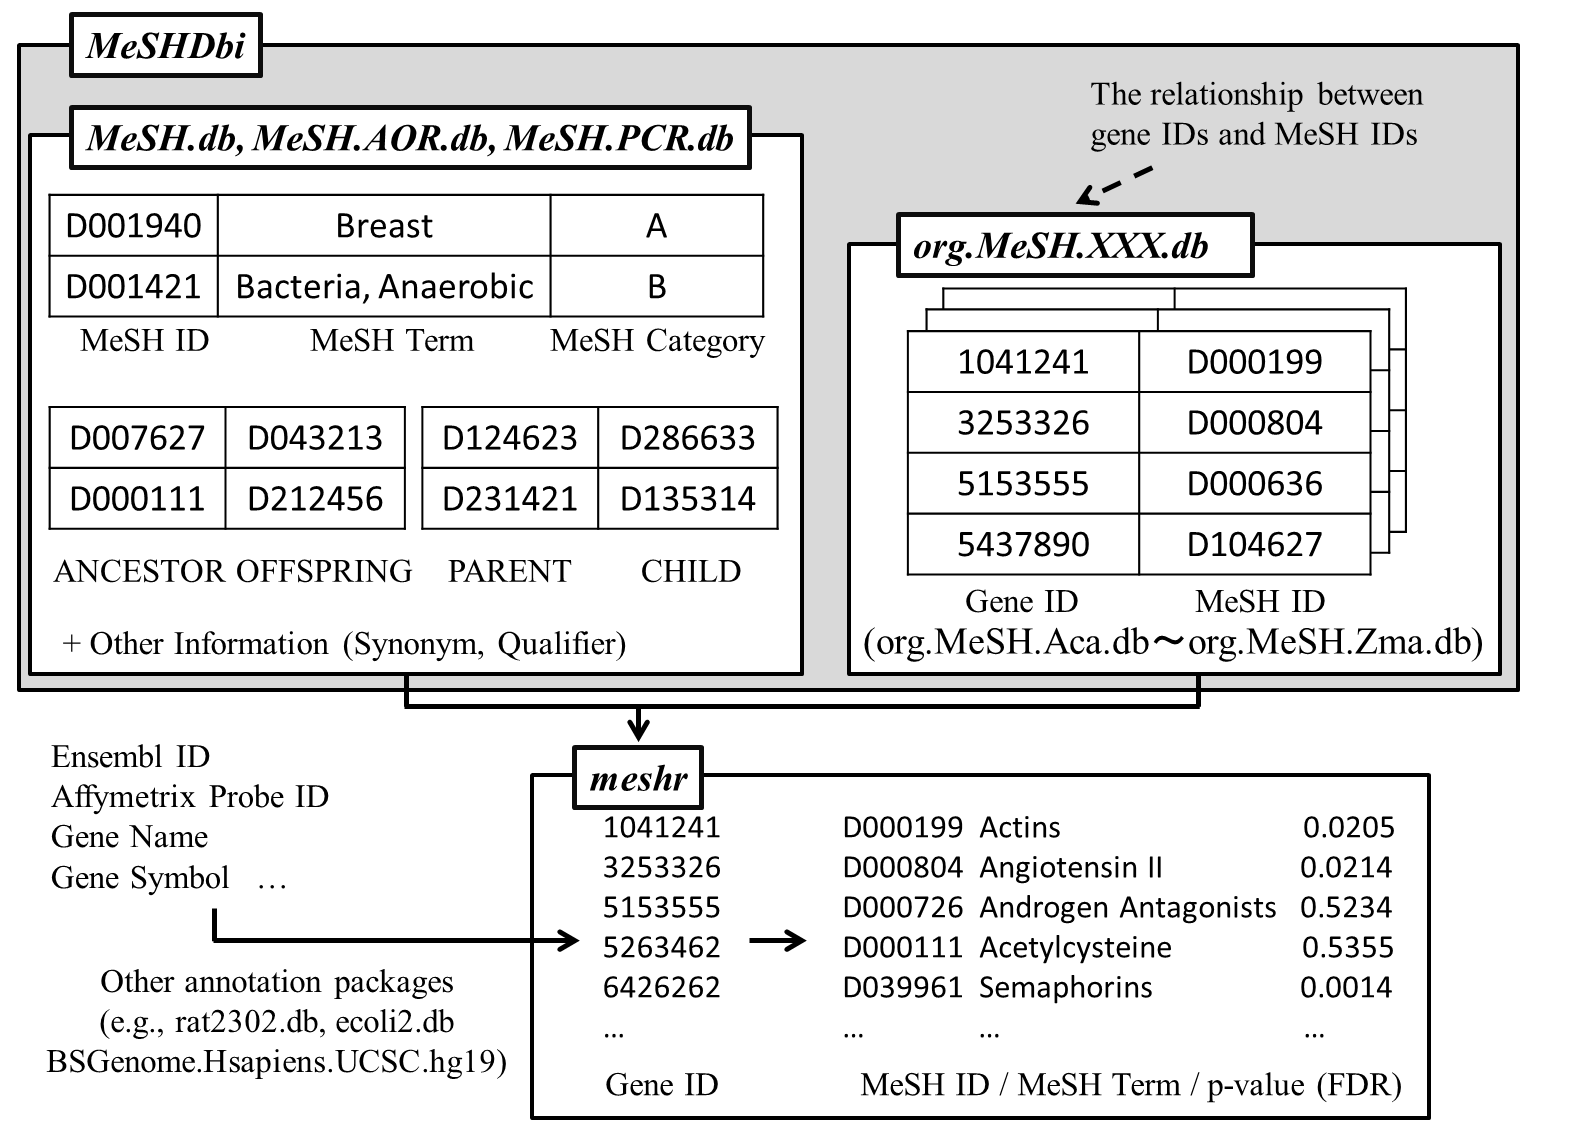
\includegraphics[width=\linewidth]{fig4.png}
\caption{The relationship of meshr and other MeSH-related packages}
\label{fig4}
\end{figure}
%%%%%%%%%%%%%%%%%%%%%%%%%%%%%%%%%%%%%%%%%%%%%%%%%%%%%%%%%%%%%%%%%%
\clearpage
\section{Exercise}
\subsection{Access MeSH Term}
\subsubsection{columns, keytypes, keys, and select}
In our packages, all data are extracted by only 4 functions defined by \Rpackage{AnnotationDbi}; $\bf{keytypes}$, $\bf{columns}$, $\bf{keys}$ and $\bf{select}$. In this section, we demonstrate how to use these functions by using \Rpackage{MeSH.db}.

At first, install and load the \Rpackage{MeSH.db}.
\begin{center}
\begin{Schunk}
\begin{Sinput}
> library(MeSH.db)
\end{Sinput}
\end{Schunk}
\end{center}

ls function shows all objects in this package. MeSH.db object is generated. This is also package's name and all MeSH-related packages provide the object named as package name (e.g., $MeSH.db$, $org.MeSH.Mmu.db$).
\begin{center}
\begin{Schunk}
\begin{Sinput}
> ls("package:MeSH.db")
\end{Sinput}
\begin{Soutput}
[1] "MeSH.db"
\end{Soutput}
\begin{Sinput}
> MeSH.db
\end{Sinput}
\begin{Soutput}
[1] "##### class ####"
[1] "MeSHDb"
attr(,"package")
[1] "MeSHDbi"
[1] "##### connection #####"
<SQLiteConnection>
[1] "##### package name #####"
[1] "MeSH.db"
\end{Soutput}
\end{Schunk}
\end{center}

Here, we use $\bf{columns}$, $\bf{keytypes}$, $\bf{keys}$ and $\bf{select}$ against MeSH.db.\\

$\bf{columns}$ returns the rows which we can retrieve in MeSH.db.
\begin{center}
\begin{Schunk}
\begin{Sinput}
> columns(MeSH.db)
\end{Sinput}
\begin{Soutput}
[1] "MESHID"      "MESHTERM"    "CATEGORY"    "SYNONYM"     "QUALIFIERID"
[6] "QUALIFIER"  
\end{Soutput}
\end{Schunk}
\end{center}

$\bf{keytypes}$ returns the rows which can be used as the optional parameter in $\bf{keys}$ and $\bf{select}$ functions against MeSH.db.

\begin{center}
\begin{Schunk}
\begin{Sinput}
> keytypes(MeSH.db)
\end{Sinput}
\begin{Soutput}
[1] "MESHID"      "MESHTERM"    "CATEGORY"    "SYNONYM"     "QUALIFIERID"
[6] "QUALIFIER"  
\end{Soutput}
\end{Schunk}
\end{center}

\newpage
$\bf{keys}$ function returns the value of keytype.
\begin{center}
\begin{Schunk}
\begin{Sinput}
> k <- keys(MeSH.db, keytype = "MESHID")